\subsection{\nue appearance in long baseline experiments and the quest for \dcp}
As mentioned in~\ref{sec:theta13}, the main goal of long baseline experiments is nowadays the search for \nue and \nueb appearance. The \nue appearance is in fact a sub-leading effect of the disappearance of muon neutrinos depending on a combination of \thint, \thatm, \dcp, and mass hierarchy as shown in Eq.~\ref{eq:theta13app}.

The \nue appearance phenomenon has been observed for the first time by T2K in 2012~\cite{Abe:2013hdq}. A total of 28 electron neutrino candidates were detected in Super-Kamiokande while $4.92\pm0.55$ background events were expected for $\thint=0$. The \ptheta distribution for these events is shown in Fig~\ref{fig:t2kapp} and the significance of this measurement correspond to $7.3\sigma$. In 2016 also the NOVA experiment has reported the observation of \nue appearance, by observing 33 e-like candidates to be compared with an expected background of 8 events (see Fig.~\ref{fig:novaapp}.

\begin{figure} [h!]
\begin{center}
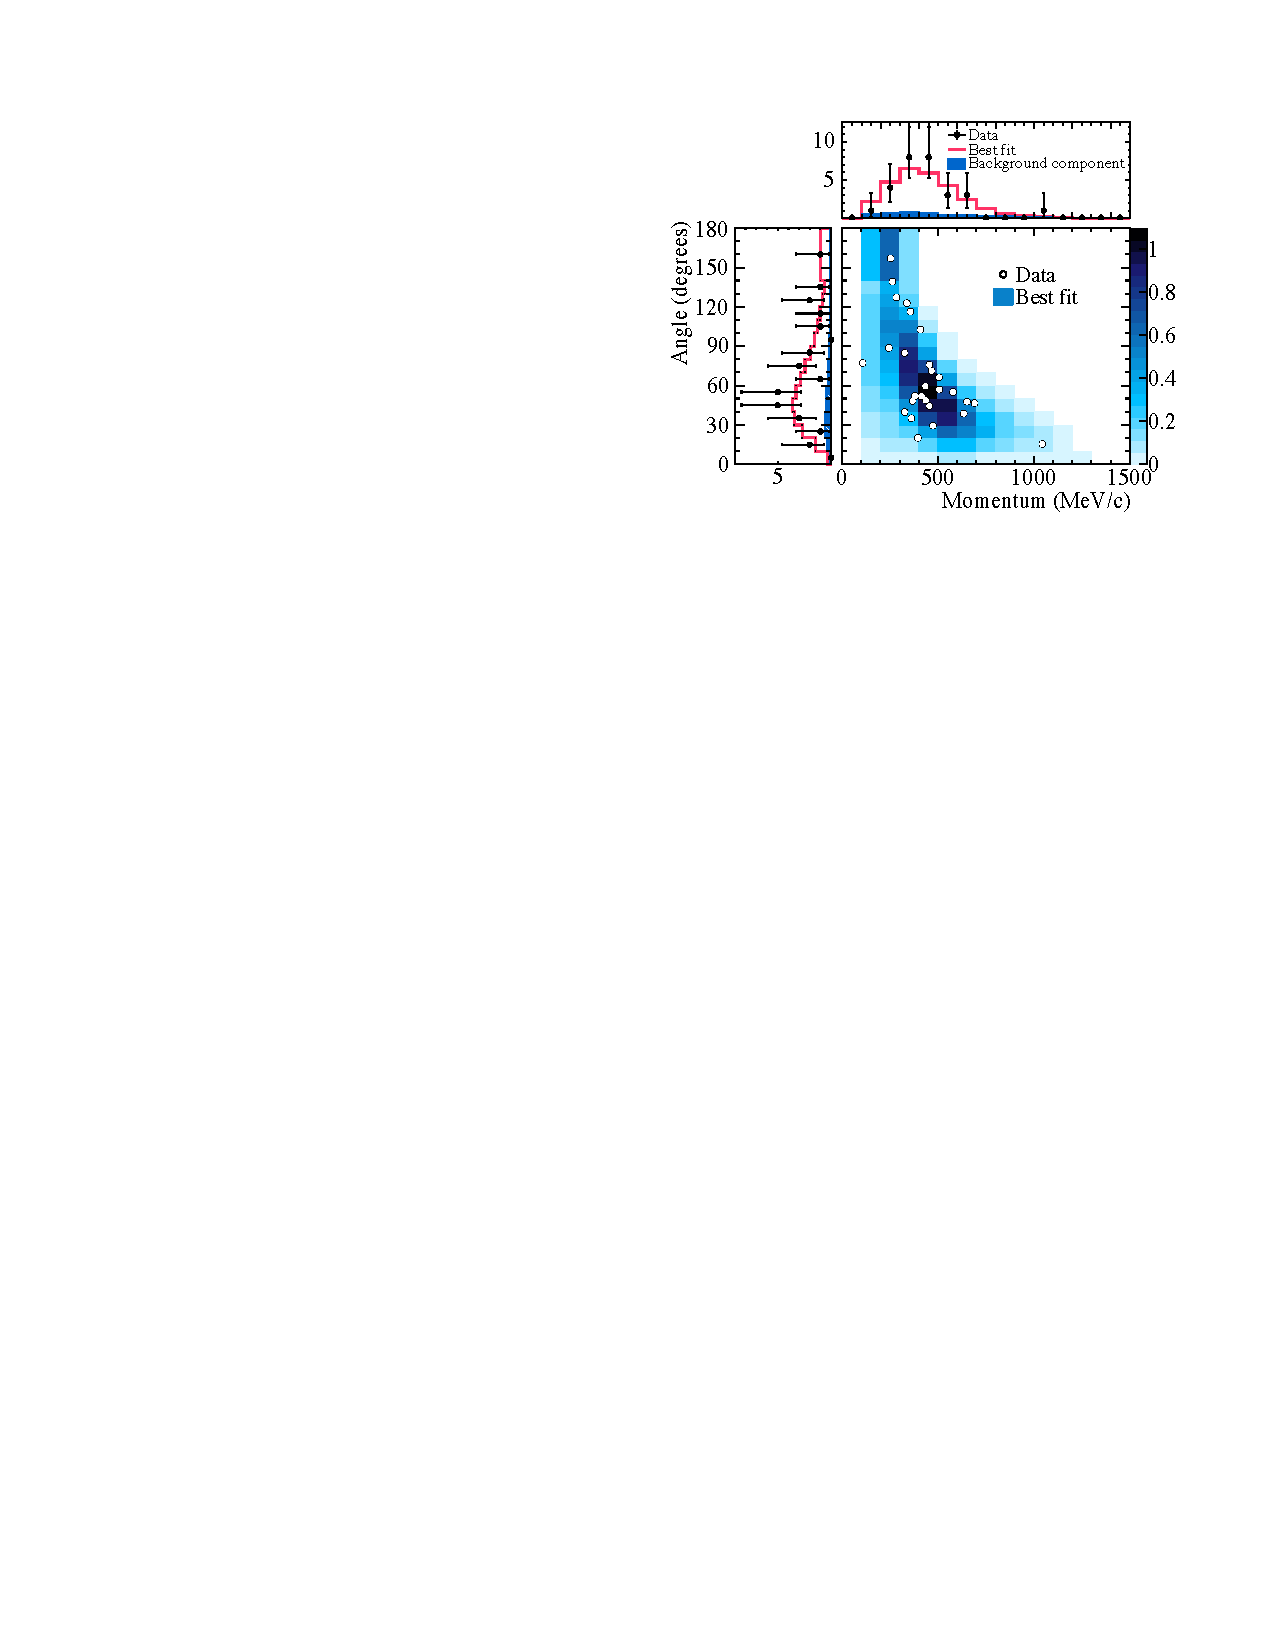
\includegraphics[width=8cm]{plotPhysics/nueapp_ptheta.pdf}
\caption{\label{fig:t2kapp} \ptheta (left) and \erec (right) distribution for the \nue candidates events~\cite{Abe:2013hdq}.}
\end{center}
\end{figure}

\begin{figure} [h!]
\begin{center}
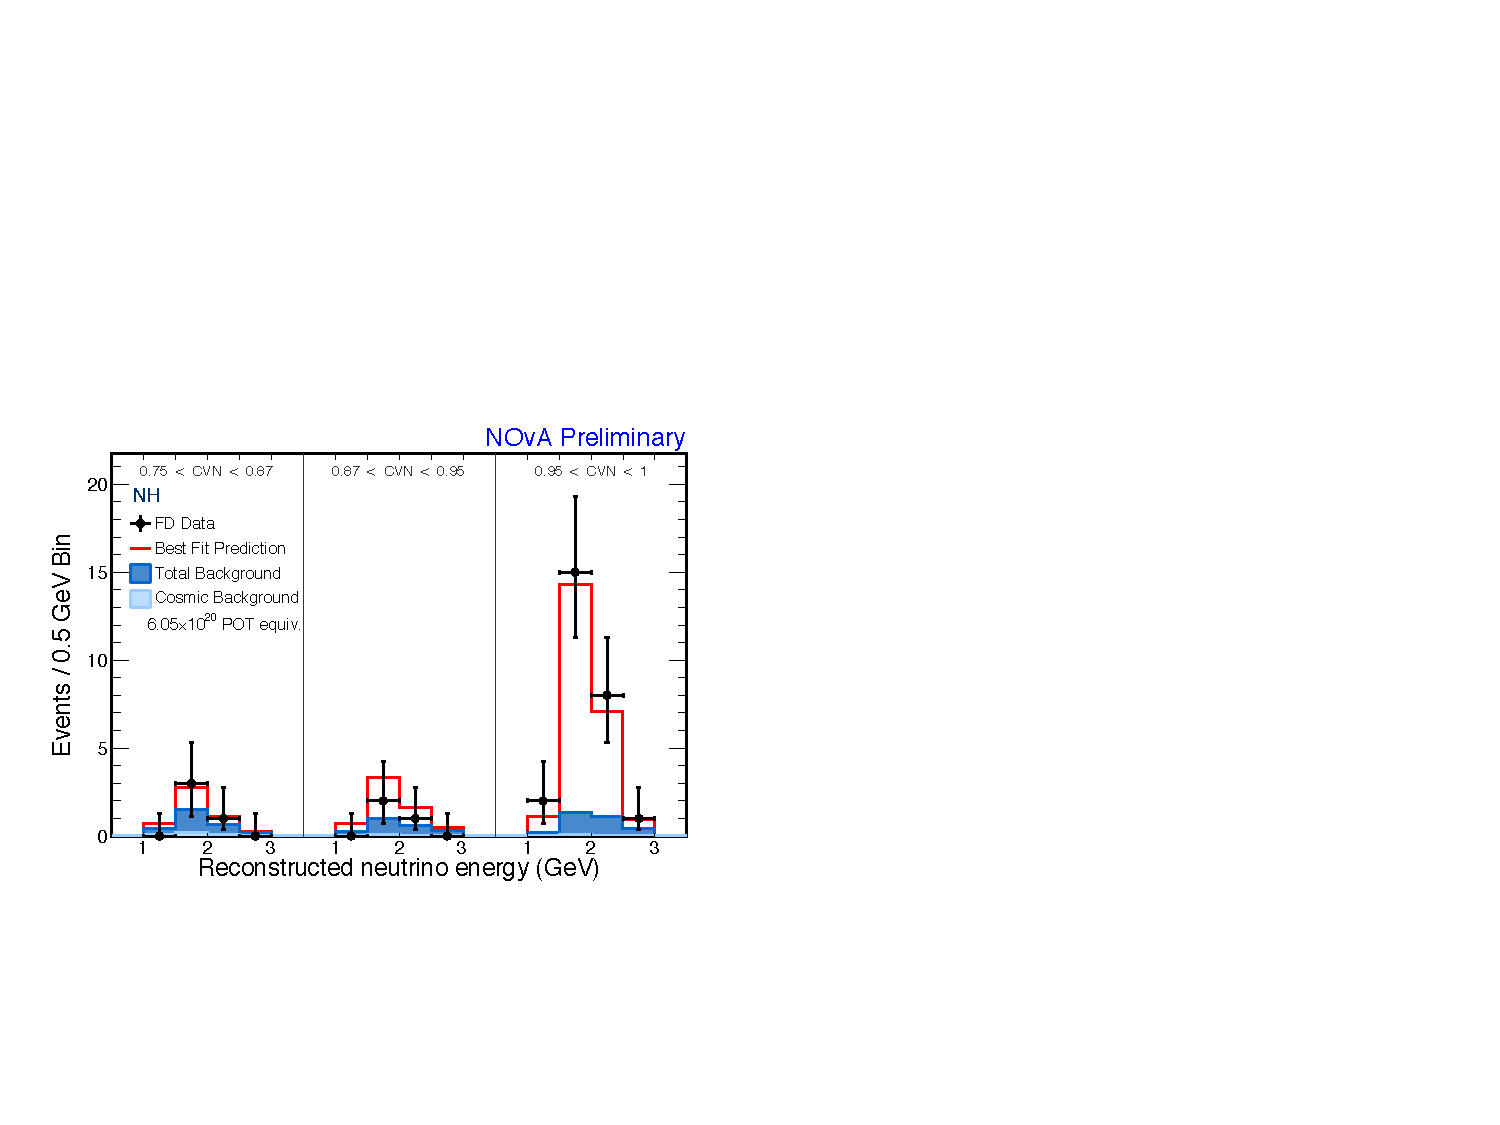
\includegraphics[width=8cm]{plotPhysics/nueapp_NOVA.pdf}
\caption{\label{fig:novaapp} \ptheta (left) and \erec (right) distribution for the \nue candidates events~\cite{Abe:2013hdq}.}
\end{center}
\end{figure}

By combining the observation of \nue apperance in long-baseline experiments with the precise measurement of \nueb disappearance with reactors it is possible to extract information on the sub-leading terms entering the appearance probability, particularly the CP violation term \dcp and the mass hierarchy sign. 
The relative size of the effect on the apperance probability due to \dcp and to the mass ordering depends on the baseline. The effect of the hierarchy is in fact proportional to the amount of matter crossed by neutrinos before reaching the detector. 

In the case of T2K the baseline is relatively short (295 km) and the matter effects contribute to $\sim\pm10\%$ of the oscillation probability while the effect due to \dcp can be as large as $\pm30\%$ for the extreme values of \dcp as shown in Fig.~\ref{fig:t2kappprob}. In the case of NOVA the baseline is 810 km and the effect of the mass ordering and of \dcp on \papp is roughly equal and it corresponds to $\sim20\%$ for each source.

\begin{figure} [h!]
\begin{center}
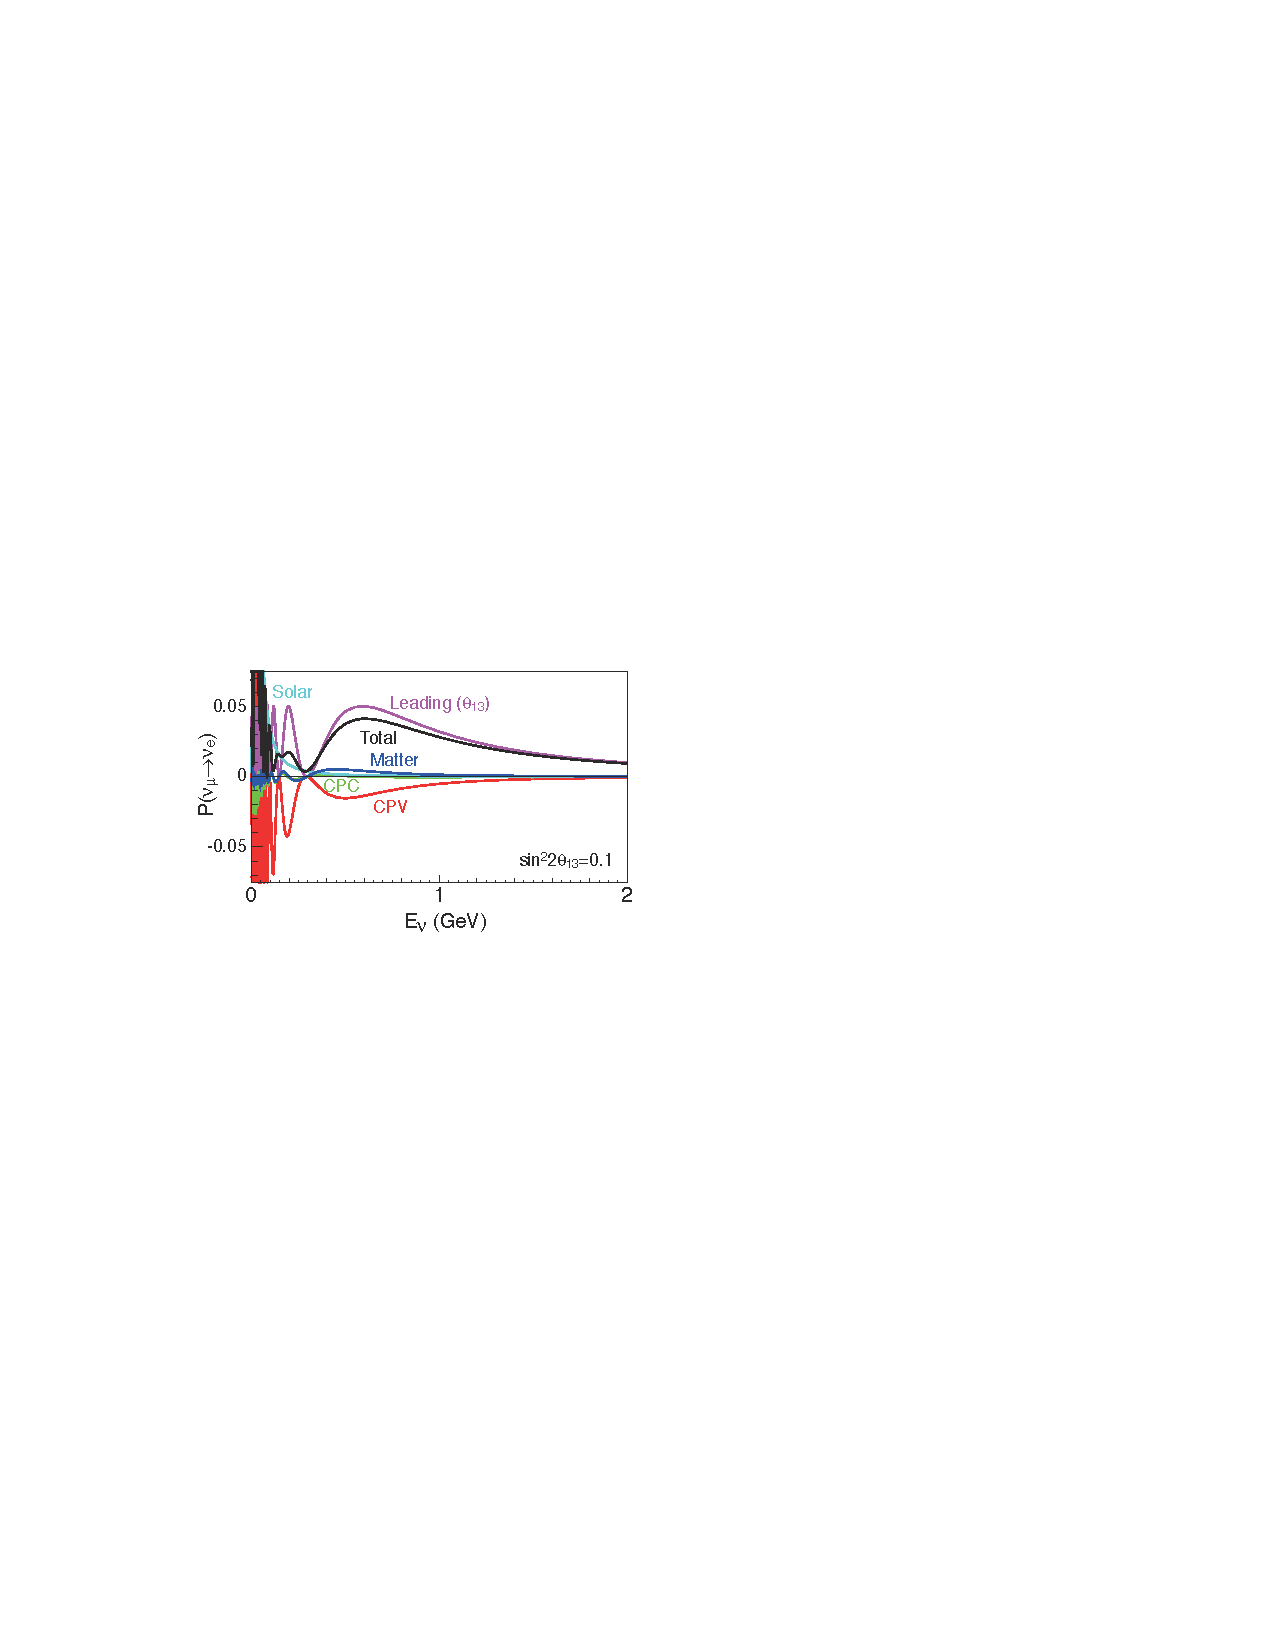
\includegraphics[width=8cm]{plotPhysics/papp_prob_2.pdf}
\caption{\label{fig:t2kappprob} Oscillation probabilities as a function of neutrino energy with L=295 km, \stot = 0.1, \dcp=$\pi/2$ and normal hierarchy. The contribution of the different terms of the oscillation probability is shown separately.}
\end{center}
\end{figure}

It is important to notice that for \nueb appearance the signs are reverted. In neutrino mode the appearance probability is maximized for normal hierarchy and $\dcp=-\pi/2$ while in anti-neutrino mode the appearance probability is maximized for inverted hierarchy and $\dcp=\pi/2$ as it is shown in Fig.~\ref{fig:t2kappnub} for the case of T2K. This figure clearly show the complementarity between \papp and \pappb and illustrates the importance of taking data also focusing anti-neutrino to fully exploit the asymmetry between \nue and \nueb apperance to measure \dcp.

\begin{figure} [h!]
\begin{center}
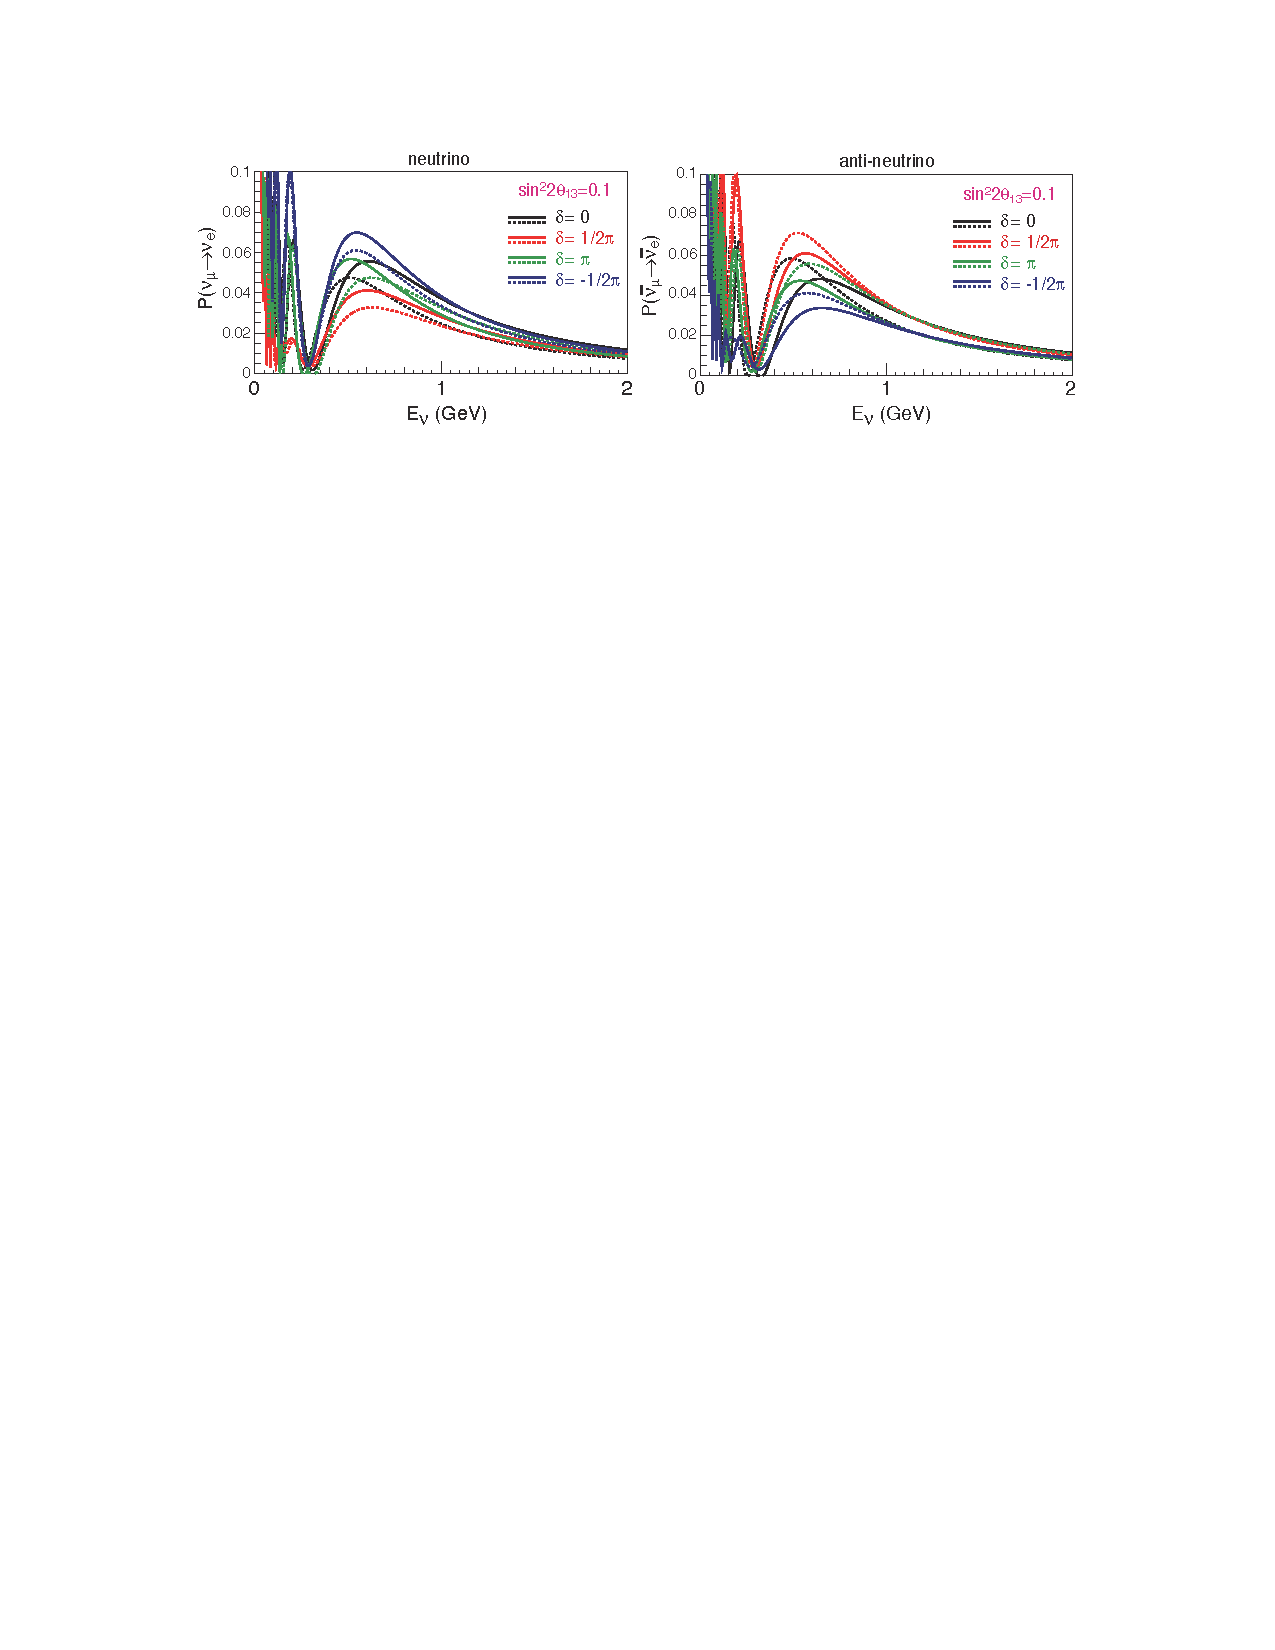
\includegraphics[width=14cm]{plotPhysics/papp_prob.pdf}
\caption{\label{fig:t2kappnub} Oscillation probabilities as a function of neutrino energy for \papp (left) and \pappb (right) with L=295 km and \stot = 0.1. The different line colors correspond to different values of \dcp while the solid (dashed) lines represent the normal (inverted) hierarchy.   }
\end{center}
\end{figure}

Finally Eq.~\ref{eq:theta13app} shows that the appearance probability also depends on the value of \thatm. Long-baseline accelerator experiments searching for \nue appearance are also sensitive to \thatm through \num disappearance. To fully take into account the correlations between oscillation parameters it is preferable to perform a joint analysis of appearance and disappearance. This procedure was used by T2K in~\cite{ } and for the most recent results presented at Neutrino2016 also the \numb disappearance and the \nueb apperarance channels are included into the same fit.
 
\subsubsection{Search for \dcp in T2K and \nova}
In the coming years, before new projects, that will be described in~\cite{sec:future}, will come online, the quest for the missing parameters in the PMNS scheme (\dcp, mass ordering, \thatm octant) will be lead by the two long-baseline accelerator experiments that are currently taking data, namely T2K and NOVA.

T2K has recently published its first analysis of neutrino oscillations obtained combining data taken with neutrinos and antineutrinos beam with approximately the same amount of POT. With this data set 32 e-like candidates are observed at SK in neutrino mode and 4 in antineutrino mode. The expected number of events depends on the value of \dcp and of the mass ordering, varying between 19.6 and 28.7 (17.1 and 25.4) for normal (inverted) ordering in neutrino mode and between 6.0 and 7.7 (6.5 and 7.4) in antineutrino mode. The maximum values of CP violation, when \dcp is equal to $\pi/2$ or $-\pi/2$ have different behavior for neutrinos and anti-neutrinos. $\dcp=-\pi/2$ maximize the \nue appearance probability and minimize the \nueb appearance probability while the opposite happens for $\dcp=\pi/2$. 

Since T2K observes a mild excess of \nue candidates even respect to the most favorable value and a deficit of \nueb candidates, a value of \dcp close to $-\pi/2$ and the normal ordering is preferred by these data even without the inclusion of the reactor constraint for the measurement of \thint. This is shown in Fig.~\ref{fig:t2kjoint}. For the first time, long-baseline experiments have sensitivity to \dcp without considering independent informations from reactors and a good agreement between the value of \thint measured by the reactors and the one measured by T2K is observed. 

\begin{figure} [h!]
\begin{center}
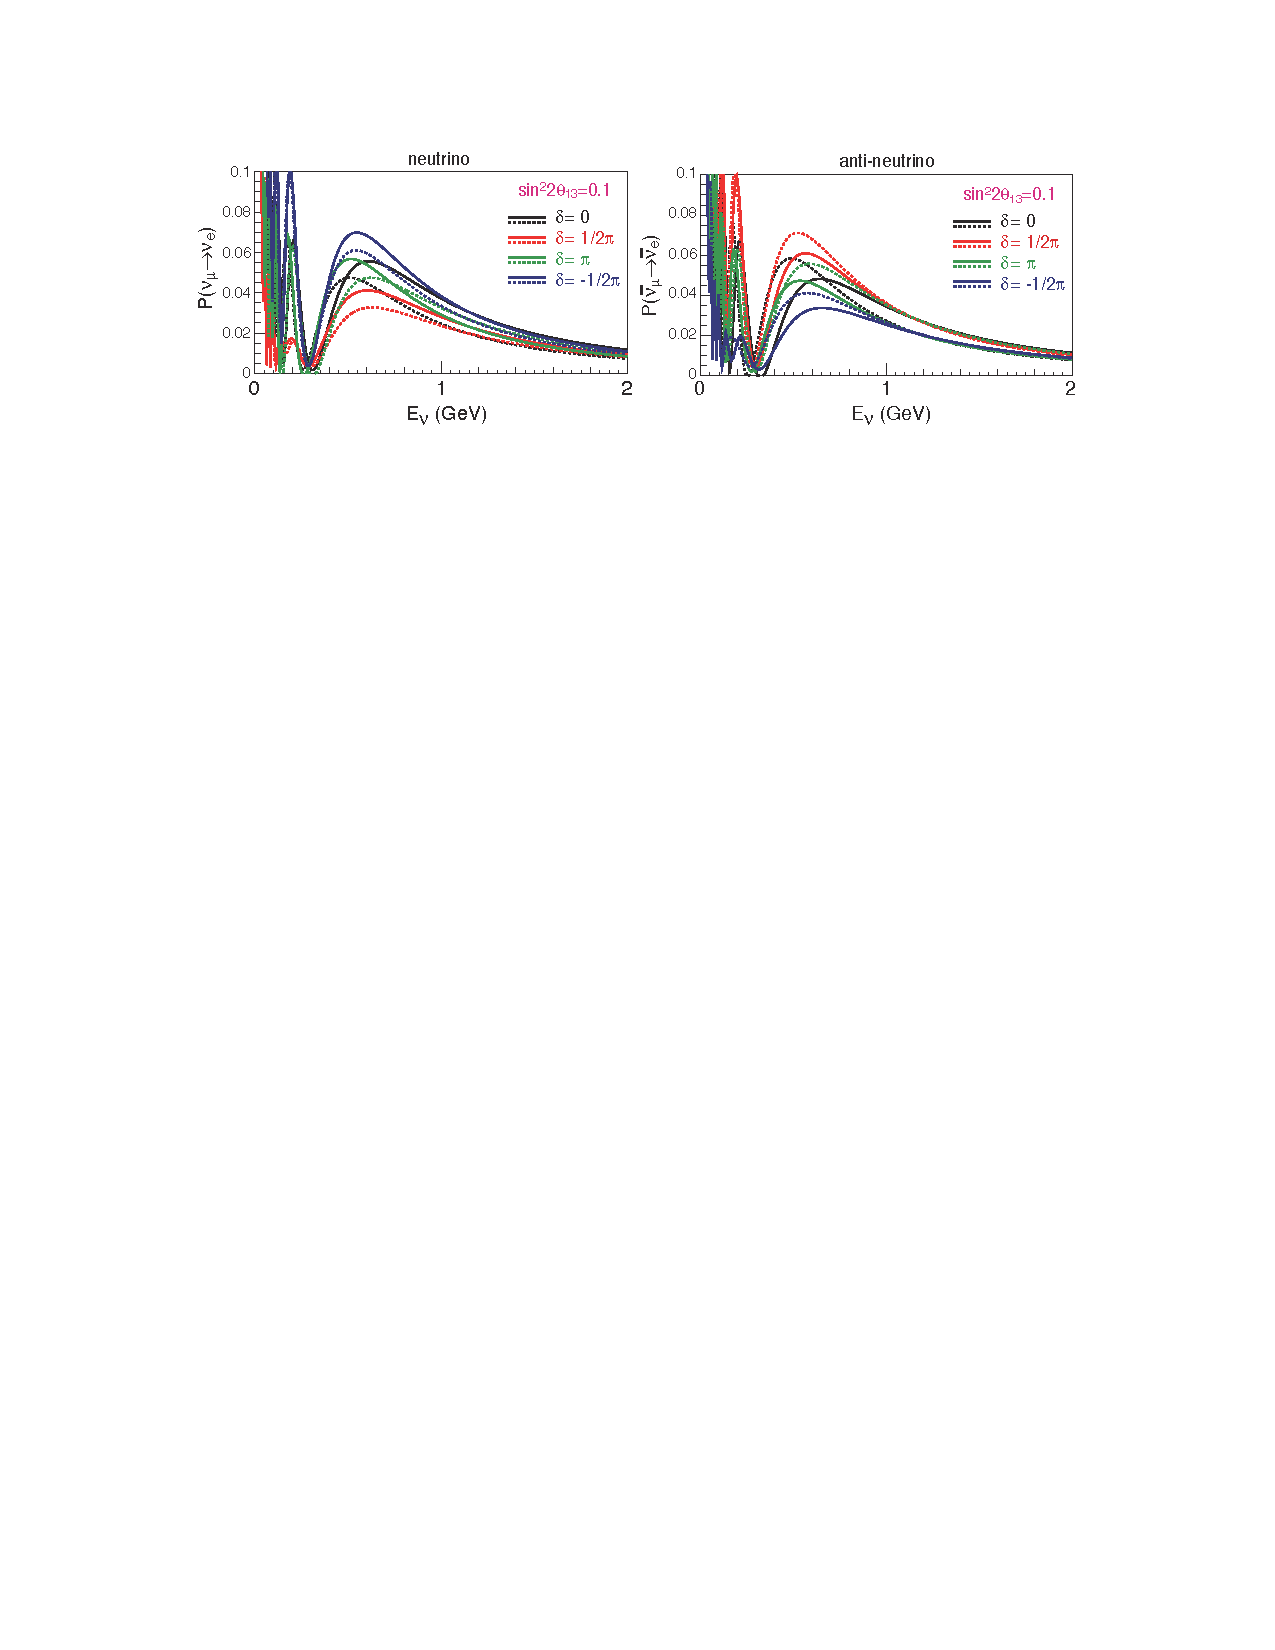
\includegraphics[width=14cm]{plotPhysics/papp_prob.pdf}
\caption{\label{fig:t2kjoint}  }
\end{center}
\end{figure}


When the average value of \thint as measured by the reactor experiments is used additional informations on the value of \dcp can be obtained. The T2K collaboration has obtained confidence intervals for \dcp using the Feldman-Cousins method (see Fig.~\ref{fig:t2kdcp}) and values conserving CP (\dcp=0 or $\pi$) are excluded at 90\% C.L.

\begin{figure} [h!]
\begin{center}
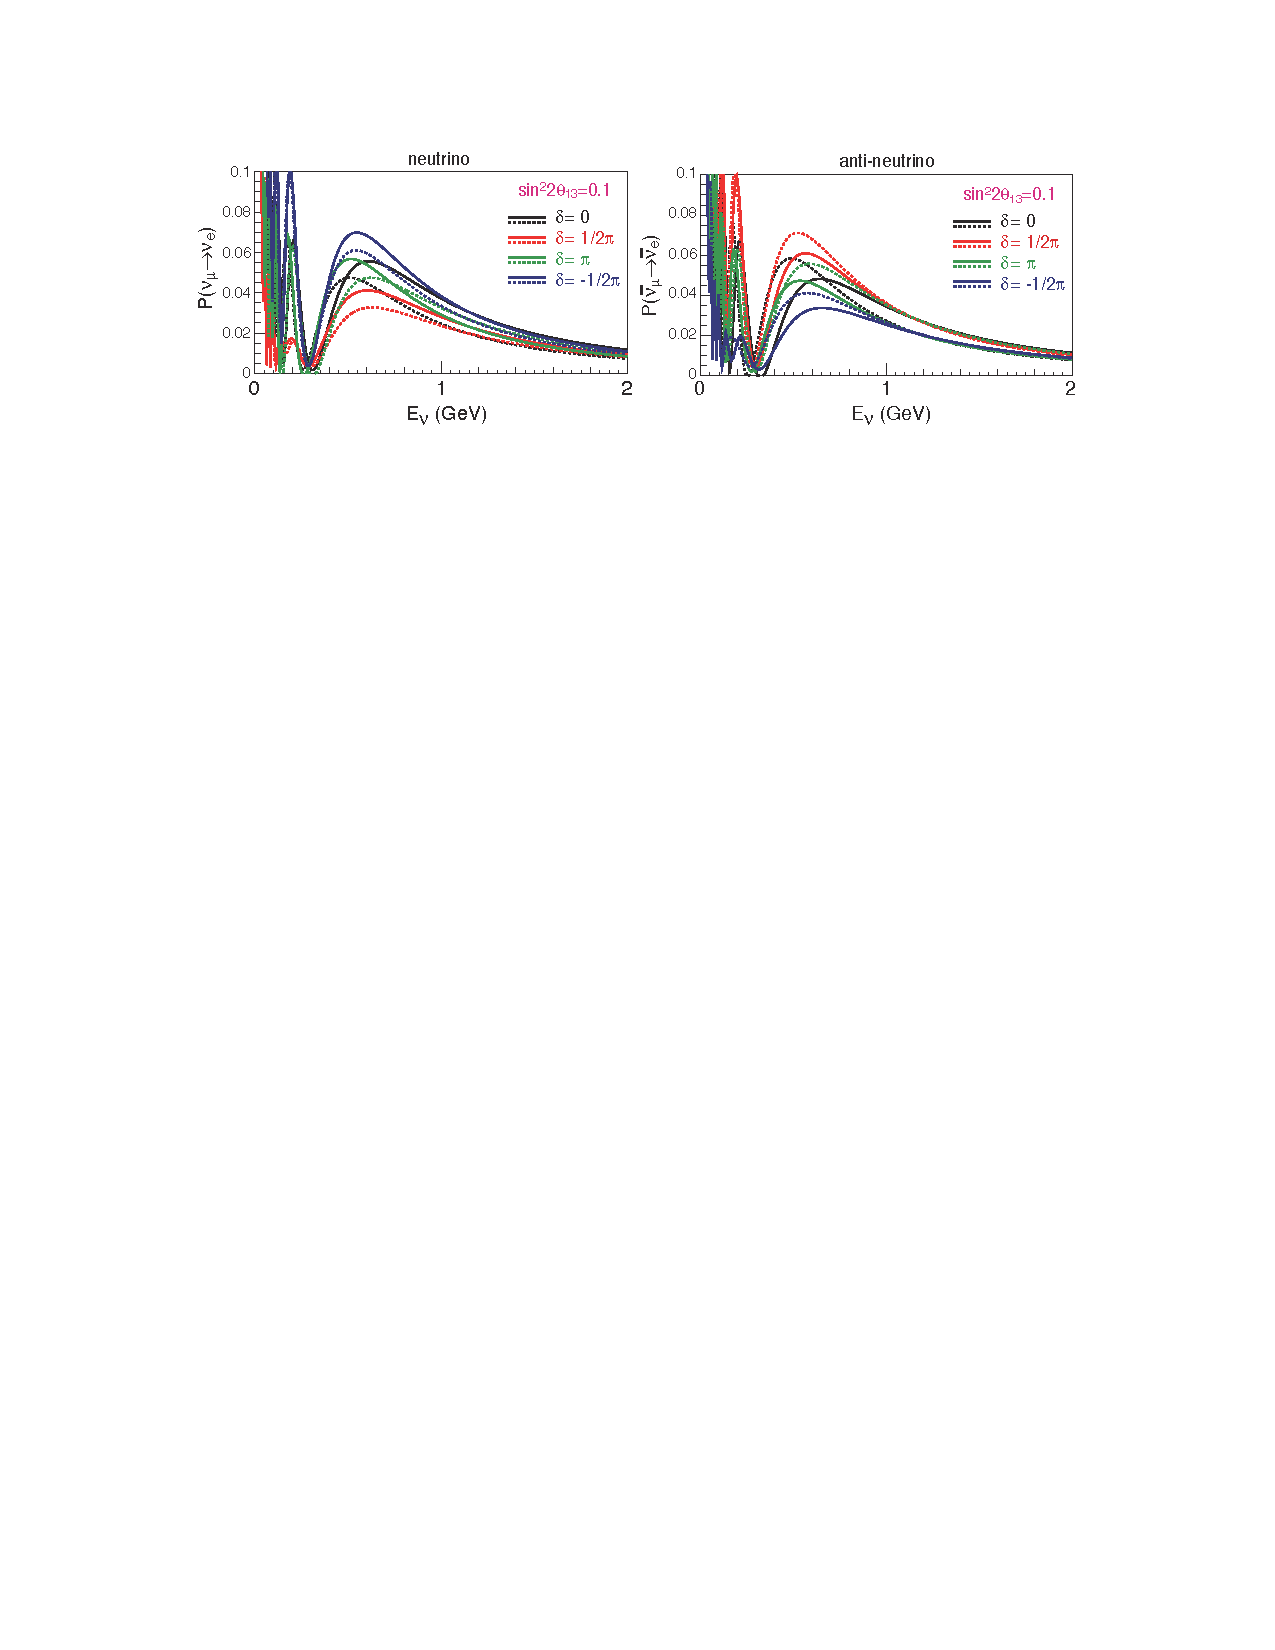
\includegraphics[width=14cm]{plotPhysics/papp_prob.pdf}
\caption{\label{fig:t2kdcp}  }
\end{center}
\end{figure}

 
\nova has also released new results for the \nue appearance (they did not collected data with antineutrino yet). They observed 33 \nue candidates events at the far detector with $8.2\pm0.8$ background events expected. The prediction for the signal events vary from 28.2 (Normal Ordering, $\dcp=-\pi/2$) to 11.2 (Inverted Ordering, $\dcp=\pi/2$). A joint analysis of appearance and disappearance channels has not been released by \nova yet but using the constraints from their own disappearance sample the results in the \stt-\dcp plane is shown in Fig.~\ref{fig:novadcp}. The data have a mild preference for normal ordering, non-maximal values of \stt. \nova foresee to start taking data in antineutrino mode in 2017 and those data will help in solving the degeneracies shown in Fig.~\ref{fig:novadcp}. 

\begin{figure} [h!]
\begin{center}
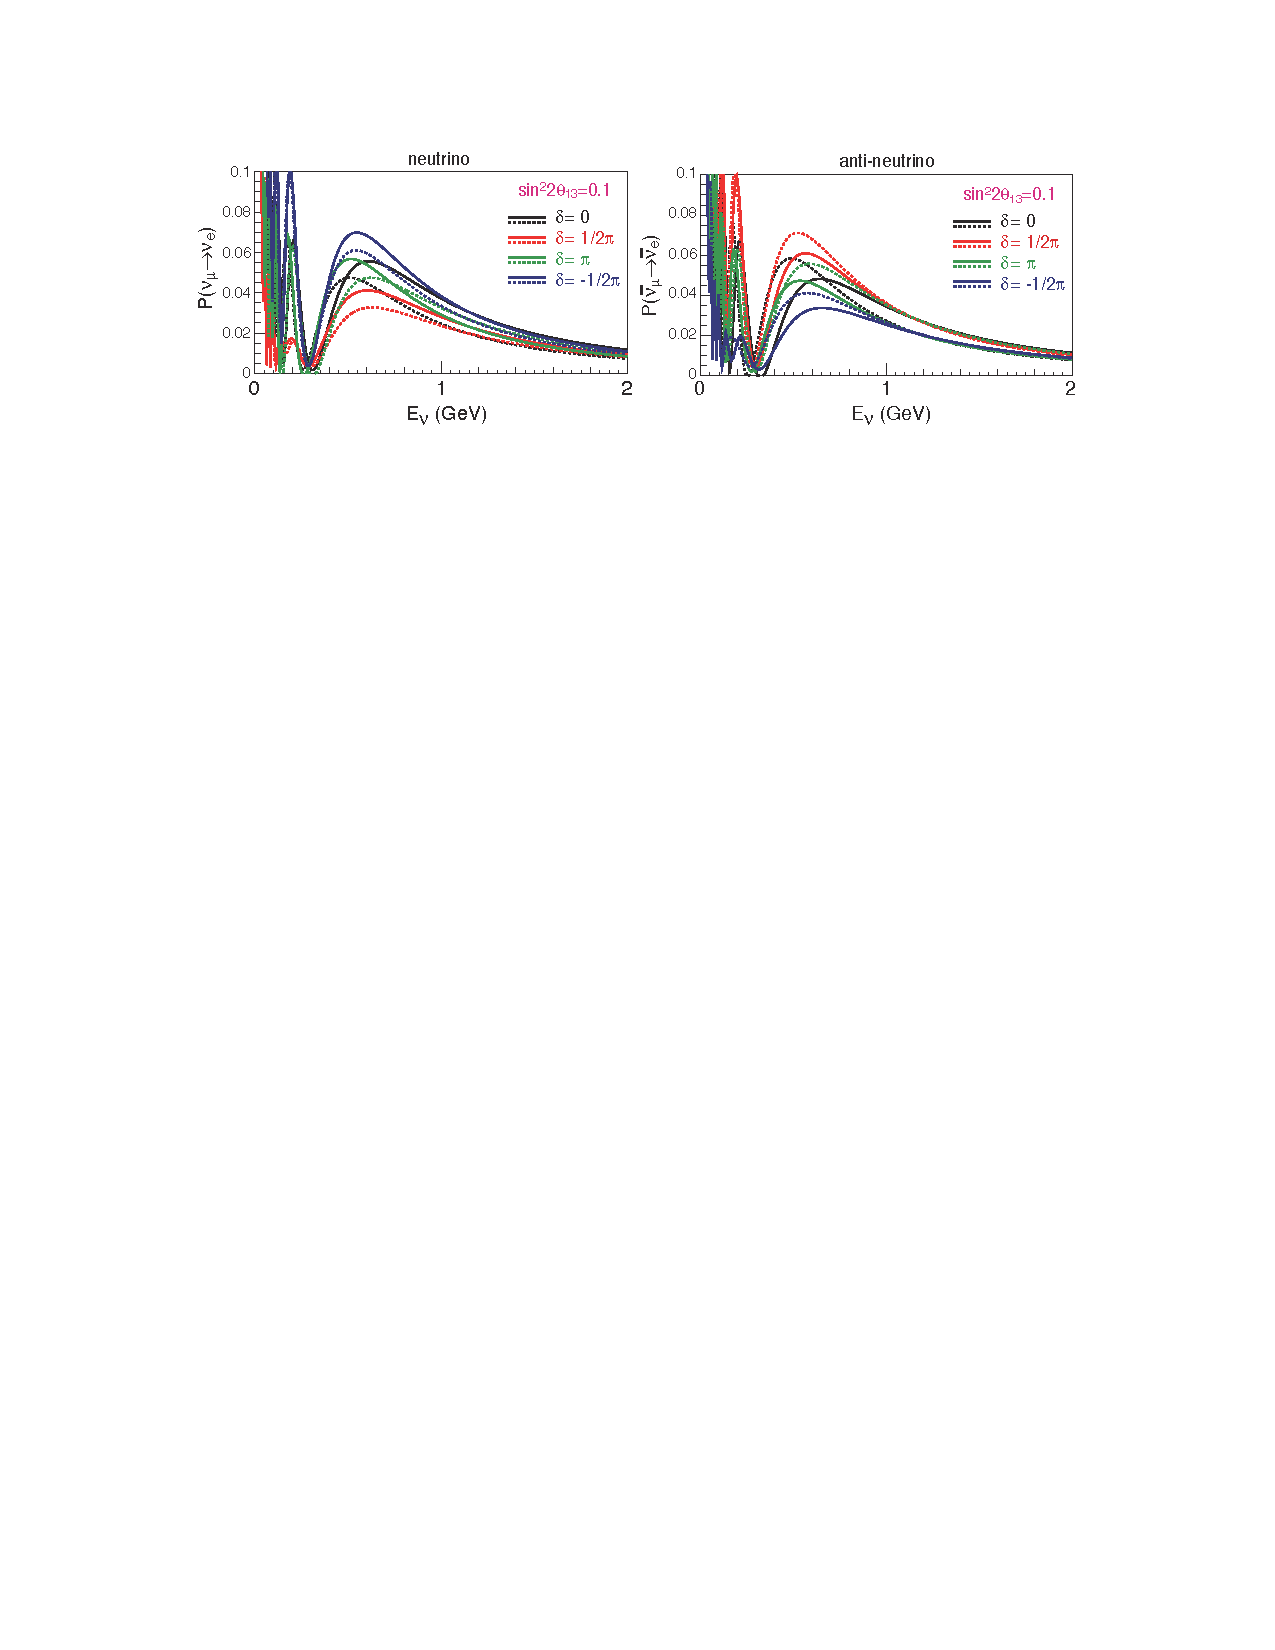
\includegraphics[width=14cm]{plotPhysics/papp_prob.pdf}
\caption{\label{fig:novadcp}  }
\end{center}
\end{figure}



\subsubsection{ Search for \dcp in Super-Kamiokande}
SK effect in atm due to delta
